\documentclass[a4paper,norsk]{article}
\usepackage{preamble}

\begin{document}
\maketitle

\section*{Introduction of problem}

In this assigment, the following exercise was presented: 

\begin{flushleft}
 Assuming potential theory in unbounded fluid, and use of Green's second identity, calculate the velocity potential along the body and the added mass forces, for a circle, an ellipse, a square and a rectangle, moving laterally, and with rotation. 
 Find also the cross coupling added mass coefficients. For the circle, the reference solution is: phi=-a*a*x/(r*r) where a denotes the cylinder radius, r*r=x*x+y*y.
\end{flushleft}

\section*{Theory}

From our study of \textbf{Green's Theorem and Distribution of Singularities} in J.N. Newmans \textbf{Marine Hydrodynamics}, the following important result where presented. \newline
By assuming potential theory, let two potentials $\phi$ and $\psi$ be solutions of Laplace's equation for a fluid in a volume 
\textbf{\textit{V}} within a closed surface \textbf{\textit{S}}. We now substitue $\psi$ with the potential for a unit source 
\textit{G}, where the source point \textbf{$\xi$} = ($\xi$, $\eta$, $\varsigma$) is either located outside, on or withing the boundary \textbf{\textit{S}}. Now we assume a body moving within the fluid, expanding the volume \textbf{\textit{V}} so the fluid can be seen as infinite and unbound. For a large spherical radius, the surfaceintegral of the boundary \textbf{\textit{S}} at infinite can be neglected, hence we only need to consider the surface where the fluid is in contact with the body.


\begin{align*}
\iint\limits_S \Big(\phi \frac{\partial G}{\partial n} - G\frac{\partial \phi}{\partial n}\Big) dS =
\begin{Bmatrix}
0 \\ -2\pi \phi(x,y,z) \\ -4\pi \phi (x,y,z)
\end{Bmatrix}
\end{align*}

\begin{align*}
G(x,y,z,\xi,\eta,\varsigma) = \frac{1}{r} + H(x,y,z,\xi,\eta,\varsigma)
\end{align*}

Where the result represents if (x,y,z) is either outside, on or inside the boundary \textbf{\textit{S}}. 
Here the function G represents a \textbf{\textit{Green Function}}, while H is a solution of the Laplace equation, and can be used to suit different types of boundary conditions. \newline 
In our assignment we are supposed to study different types of geometry in 2D, the relation then yeilds 

\begin{align*}
\iint\limits_S \Big(\phi \frac{\partial G}{\partial n} - G\frac{\partial \phi}{\partial n}\Big) dS =
\begin{Bmatrix}
0 \\ -\pi \phi(x,y,z) \\ -2\pi \phi (x,y,z)
\end{Bmatrix}
\end{align*}
Where \textbf{\textit{S}} now is the surface of our 2D geometry \newpage



\section*{Numerical Approach}
We take a closer look at our line integral, where we want to evaluate (x,y) on the surface \textbf{\textit{S}}. Here we will take S to be a circle, which has been numerical implemented of several segments \textit{$C_s$}

\begin{align*}
-\pi \phi(x_0) = \int\limits_S \Big(\phi \frac{\partial \psi}{\partial n} - \psi \frac{\partial \phi}{\partial n} \Big) dS
\end{align*}

Here $\psi$ = ln r, which is the source potential in 2D. Furthermore, we consider $\phi$ and $\frac{\partial \phi}{\partial n}$ to be constant on each linesegment.

\begin{align*}
\pi \phi(X_0) + \sum_{n=1}^N \phi(X_n) \int\limits_{Cs} \frac{\partial}{\partial n} ln r \hspace{1mm}dS = 
\sum_{n=1}^N \frac{\partial \phi}{\partial n_{X}} \int\limits_{Cs} ln r \hspace{1mm} dS
\end{align*}
Taking a closer look on our integral in the second term, we exploit a trick with complex numbers. Using the relations

\begin{align*}
ln(z) &= ln(r e^{i\theta}) = ln\hspace{1mm}r + i\theta \\
ds &= \sqrt{dx^2 + dy^2}\hspace{1mm}; n_2\hspace{1mm}dS = dx \hspace{1mm}; -n_1 dS = dy  \\
\int\limits_{Cs} \frac{\partial}{\partial n_x} ln r \hspace{1mm}dS &= 
Re \int\limits_A^B \big(n_1 \frac{\partial}{\partial x}  + n_2 \frac{\partial}{\partial y} \big)
ln \hspace{1mm}z \sqrt{dx^2 + dy^2} = 
Re \int\limits_A^B \frac{n_1+in_2}{z}\sqrt{dx^2 + dy^2} \\
&= Re \int\limits_A^B \frac{-dy+idx}{z}\sqrt{dx^2 + dy^2} = Re \hspace{1mm}i\int\limits_A^B \frac{dz}{z} =
Re \Big(i \hspace{1mm} ln \hspace{1mm}z \Big|_A^B \hspace{1mm} \Big) \\
&= -\Big(\theta_B - \theta_A \Big)
\end{align*}
Hence the integral can be interpreted as the angle between the node points where each potential is located. It is important to understand that each potential is seen as the average between the node points, and therefore located as ghost point between the node points. For our last integral we look at
\begin{align*}
\sum_{n=1}^N \frac{\partial \phi}{\partial n_{X}} \int\limits_{Cs} ln r \hspace{1mm} dS
\end{align*}x

Again it is important to notice that we operate with two reference systems. Firstly the term $\frac{\partial \phi}{\partial n_{X}}$ is the normal component of $\phi$ at the line segment, where the normal vector is on that line segment. On the other hand the coordinate $r = \sqrt{(x-x')^2 + (y-y')^2}$, we let the coordinates $(x,y)$ be fixed, and move around the geometry with
$(x',y')$. Hence each integral the $ln \hspace{1mm} r$ part is taken with respect from the $\phi$ beeing calculated on that perticular line segment. We are only interested in lateral and with rotaton in 2D. We use the relation  
\begin{align*}
\frac{\partial \phi_i}{\partial n} = n_i \hspace{5mm} i = 1, 2; \hspace{5mm} 
\frac{\partial \phi_i}{\partial n} = (\textbf{r'} \times \textbf{n})_{i-3} \hspace{5mm} i = 6 \\
\frac{\partial \phi_1}{\partial n} = n_1 = cos\theta = \frac{x}{r} \hspace{1cm}  
\frac{\partial \phi_6}{\partial n} = (\textbf{r'} \times \textbf{n})_{3}
\end{align*}  

Our goal now is to end up linear system on the following form

\begin{align*}
\begin{Bmatrix}
\pi \hspace{5mm} (\theta_1 - \theta_2) \hspace{5mm} (\theta_2 - \theta_3) \cdots \\
(\theta_{N-1} - \theta_N)  \hspace{5mm} \pi \hspace{5mm}(\theta_1 - \theta_2) \cdots \\
(\theta_{N-2} - \theta_{N-1})  \hspace{5mm} (\theta_{N-1} - \theta_N) \hspace{5mm} \pi \cdots \\
\vdots 
\end{Bmatrix}
\begin{Bmatrix}
\phi(x_0) \\
\phi(x_1) \\
\phi(x_2) \\
\vdots \\
\phi(x_N)
\end{Bmatrix}
=
\begin{Bmatrix}
\frac{\partial \phi}{\partial n} \int\limits_{C1} ln r_1 \hspace{1mm} dS \\
\frac{\partial \phi}{\partial n} \int\limits_{C2} ln r_2 \hspace{1mm} dS \\
\vdots \\
\frac{\partial \phi}{\partial n} \int\limits_{CN} ln r_N \hspace{1mm} dS
\end{Bmatrix}
\end{align*} 
By exploiting the relations presented above into the integrals, we are able to calculate the \textit{added mass tensor}
\begin{align*}
\begin{Bmatrix}
m_{11} \hspace{5mm} m_{12} \hspace{5mm} m_{16} \\
m_{21} \hspace{5mm} m_{22} \hspace{5mm} m_{26} \\
m_{61} \hspace{5mm} m_{62} \hspace{5mm} m_{66}
\end{Bmatrix}
\end{align*}
We can argue that because of lateral movement
\begin{align*}
\begin{Bmatrix}
m_{11} \hspace{5mm} 0 \hspace{5mm} 0 \\
0 \hspace{5mm} m_{22} \hspace{5mm} 0 \\
0 \hspace{5mm} 0 \hspace{5mm} m_{66}
\end{Bmatrix}
\end{align*}



\section*{Results}
\begin{figure}[h!]	
	\centering
	\caption*{Numerical approximation of m11, Circle N=1000}
	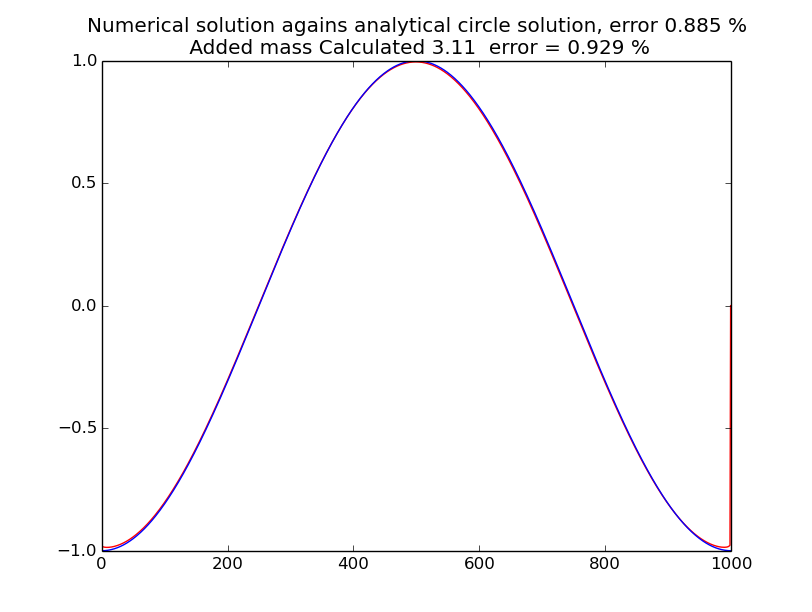
\includegraphics[scale=0.6]{circlem11.png}
\end{figure}
For a circle, the numerical results are very good. We end up with a relative error of 0.885 \% for the velocity potential on the boundary of the circle. For the added mass in lateral direction $m_{11}$, we end up with a relative error of 0.929 \%. These results gives a good indication that the numerical estimation for the circle is pretty accurate. For the yaw $m_{66}$, we execpt the analytical solution to be 0, due to the cross product $\textbf{r'} \times \textbf{n}$ is zero for a circle. This is verified from the numerical calculation

\begin{lstlisting}[style=terminal]
Exact value: 0.00000, Calculated mass: 0.00000
\end{lstlisting} \newpage
For the rest of the numerical calculations the results will be compared up against the added mass tensor, due to the lack of an exact analytical solution for the velocity potensial. \\
For an ellipse \[ \big(\frac{x}{a}\big)^2 + \big(\frac{y}{b}\big)^2 = 1   \]
I have chosen $a=1, b=3$, and as for the circle, N = 1000 elements have been chosen for good precition. The analytical solution of the \textit{mass tensor} components are presented in newman as

\begin{itemize}
\item{} $m_{11} = \rho \pi b^2$
\item{} $m_{66} = \frac{1}{8}\rho \pi(b^2-a^2)^2 $
\end{itemize}  
A run of the numerical program gives the following result for the tensor components

\begin{lstlisting}[style=terminal]
Exact value: 28.27433, Calculated mass: 27.94521, error: 1.16402 %
Exact value: 25.13274, Calculated mass: 25.03932, error: 0.37172 %
\end{lstlisting} 
With a relative error at the most $\approx$ 1\%, these are some satisfying results, pointing in the direction of a decent numerical implementation.

\section*{Conclusion}
With help from the analytical solutions, I conclude that the implementation is decent for the presented problem. The relative error is small, which conclude a valid implementation. I take criticism in implementing to many for-loops, which results in long runtime of the program for large N. I will try to implement a vectorized implementation for my next assignment.
\newpage
\lstinputlisting[style=python]{oblig1.py}

\end{document}